\documentclass{beamer} \usepackage{pgfpages} \setbeamertemplate{bibliography item}{\insertbiblabel}
\vfuzz 10pt
\usepackage{hyperref}
% UNCOMMENT FOR FINAL COMPILATION WITH SPEAKER NOTES

%\setbeameroption{show notes on second screen=right} % Both
%\setbeamertemplate{note page}{\pagecolor{yellow!5}\insertnote}\usepackage{palatino}


\usepackage{graphicx}
\graphicspath{{images/}}


\author{Sam Barrett, 1803086}
\title{{Applications of genetic algorithms on fully-autonomous road networks} \\ \texorpdfstring
        {
\includegraphics[scale=0.09]{uobcrest.jpg}} \\\\ \href{https://youtu.be/2QAttxzLam0}{$\rightarrow$Video Link$\leftarrow$}
    }
\institute{{University of Birmingham}}
\date{\today}

\begin{document}

\begin{frame}
\titlepage
\end{frame}

\section{My Topic}
\begin{frame}{My Topic}
    \note{

        \begin{itemize}
            \item I am choosing to focus on the applications of Genetic Algorithms on Theoretical Fully autonomous road networks, with a view to extend into the possible applications of quantum computers on the field in the future. 
            \item  I feel the advent of fully autonomous road networks is a logical next step in making roads safer and more efficient through the use of technology.
            \item Fully autonomous driving trials have been legal in parts of the states for years with the UK following soon.
            \item Most research and all currently implemented systems focus on semi-autonomous environments whereby self-driving vehicles and humans co-exist on shared roads. 
            \item I propose it is both safer, easier and more efficient to implement, fully autonomous road networks where humans are not able to operate their vehicles.
            \item In such a system, sensor data would be shared between all vehicles near instantaneously allowing for much faster and less-selfish route planning, leading to net decreases in travel time. 

        \end{itemize}
    }

    \begin{itemize}

        \item Semi-autonomous vehicles are becoming more prevalent 
        \item Roads are becoming more congested with a 78\% increase in motor traffic since 1993 \cite{HighwaysEnglandNetwork2015}
        \item Fully autonomous vehicle trials have been legal in parts of the US since 2015\cite{AutonomousVehiclesSelfDriving}, with the UK set to follow by next year (2021)\cite{unknownUKWantsFully2019}
        \item Much of the current research into autonomous vehicle routing focuses on environments where human drivers are still present
        \item By removing the human element and working on theoretical \textit{fully autonomous road networks} we can make many useful assumptions about the behaviour of other vehicles
        \item The solution to road congestion is not to build bigger roads, it is to optimise the traffic flows.
        \item Just 78.2\% of journeys on the UK Highway Agencies roads were \textit{on time} in the year ending June 2014 \cite{measures02079443095ReliabilityJourneysHighways}

    \end{itemize}
\end{frame}

\begin{frame}
    \note{ 
        On a theoretical level, there are a few distinct systems and algorithms that need to be implemented to create such a system:

        \begin{itemize}
            \item I will require a method of representing vehicle routes in a coordinate space, beyond a list of coordinate points. 
            \item A function that takes a route as a list of points and maps it to our genome, i.e. unpacks it into a string of Real values. 
            \item A function to facilitate the reverse, converting the string of real values back into a usable route of points.
            \item I will need to devise and implement a fitness function. This function will be the objective function of the GA and so needs to reward good solutions without causing early convergence. It also needs to be able to identify and sufficiently penalise infeasible solutions. Such as routes that leave the road space or intersect with obstacles or other routes.
            \item It will also require the implementation of various genetic operators including Selection, crossover and mutation
            \item finally we will require a utility function to verify that all newly generated individuals are valid and repair those who are not.

        \end{itemize}
    }
    \begin{figure}[htpb]
        \centering
        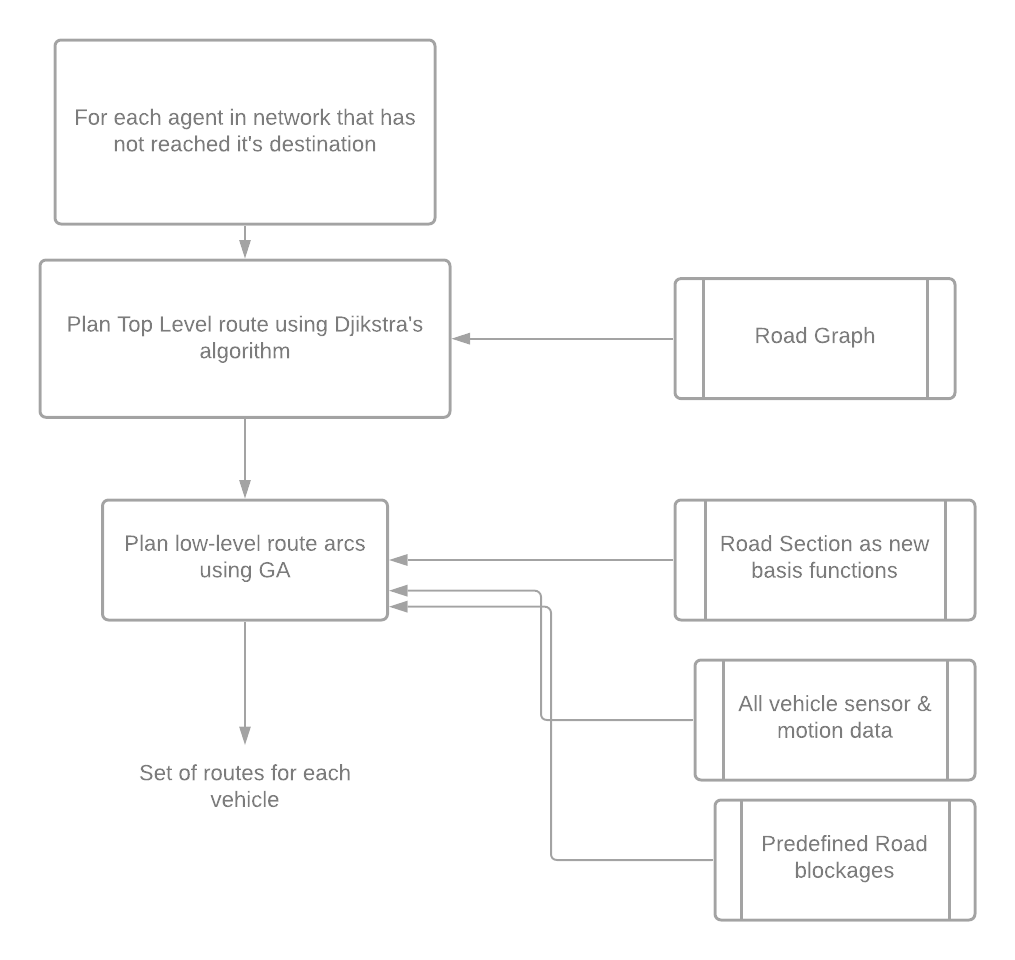
\includegraphics[width=0.3\linewidth]{ProjectTopology.png}
        \caption{Abstract Project Topology}%
        \label{fig:ProjectTopology}
    \end{figure}
    \begin{itemize}
        \item From a technical perspective, there are many things that need to be implemented to make such a system possible. 
            \begin{itemize}
                \item The functional representation of vehicle trajectories
                \item The encoding of routes into a real-valued string of genes
                \item The decoding of a real-valued string of genes to a route which a vehicle can take
                \item The implementation of a function to determine the fitness of an individual route. 
                \item Implementation of genetic operators: Selection, crossover and mutation.
                \item Cleanup operators to make certain any new individuals are valid
            \end{itemize}
    \end{itemize}

\end{frame}

\begin{frame}{My Goal}

    \note{
        \begin{itemize}
            \item My goal with this project is to investigate the viability of a fully autonomous road network using GAs for route planning 
            \item I will implement an experimental version in a programming language. This system will be implemented in a vacuum, meaning it will not interface beyond the scope of the abstract route planning. It will be assumed to have all required information including positions and sensor data from all nearby agents.
        \end{itemize}
    }

    My goal with this project is to investigate the feasibility of such a system. 

    To do so I will \textit{programatically} implement an experimental version, making various assumptions about the data available to it.

    With my system I hope to be able to run various simulations to determine it's performance in quasi real-world scenarios and conclude as to whether the use of GAs have merit in this area. 

    Currently the research yields no such results. The feasibility of similar systems have been discussed\cite{kalaOnroadIntelligentVehicles2016} but never experimentally investigated.
    
\end{frame}

\section{Literature}
\begin{frame}

    \note{
       \begin{itemize}
            \item As previously mentioned most current research into Genetic Algorithm \textit{(GA)} applications within the vehicle industry has a very broad scope. 
            \item Designing possible solutions that would fit into the current road networks easily. 
            \item I am intending to focus on a much more aspirational system, specifically looking at theoretical autonomous Motorways. 
            \item This enables me to overhaul the current road layout which was designed to aid human drivers not the overall efficiency of the system.
        \end{itemize}
        I have chosen to focus on GAs as opposed to other possible AI veins for a few reasons. 
        \begin{itemize}
            \item One personal reason is that I find them particularly interesting. 
            \item One more concrete reason is that they have the very useful property of being both probabilistically optimal and probabilistically complete. Meaning that given infinite time they not only will find \textit{a} solution but they will find \textbf{the} optimal solution. 
            \item And finally they have seen relatively minimal research in the field of vehicle planning with the limelight being taken by technologies such as Deep Learning or Reinforcement Learning
        \end{itemize}


    }

    \frametitle{Literature Review}
    I am currently intending to pursue my research assuming the absence of classical speed lanes as described by Kala and Warwick in \cite{kalaMotionPlanningAutonomous2015}. 

    I have chosen to focus on the applications of Genetic Algorithms on the field for 3 reasons: 
    \begin{enumerate}
        \item It is a class of optimisation algorithms that I find particularly interesting

        \item GAs are \textit{probabilistically optimal and complete}, i.e given infinite time, they will always produce the global optimal solution if such a solution exists\cite{kalaMotionPlanningAutonomous2013}

        \item It is a class of algorithm that has seen relatively minimal research in my specific sub-area 
    \end{enumerate}
\end{frame}

\begin{frame}

    \note{
        \begin{itemize}
            \item A many of the technologies being researched with regards to vehicular planning suffer from the same problem from my point of view, they are \textit{black box approaches} meaning given a model, it is very difficult, if not impossible, to reason about and predict the decisions it makes. Such systems could end up making decisions based on imperfections in the training set. Such issues will make these systems less dependable and make people less likely to put their faith in them.
            \item In a paper from 2013, Kala and Warwick proposed a method of representing roads as a set of boundary functions in Cartesian space. All points on the road are defined using these functions as a new basis, this seems to be a good approach as it eliminates the possibility of plotting routes outside of the road space.

    \item in a book by Kala published in 2016, 3 years after his initial paper on autonomous planning, he talks about the possibility of planning using GAs to optimise Bézier curves. Each curve is determined by $n$ control points allowing for complex motions to be abstracted to a single objective function.
        \end{itemize}



    }


    \begin{itemize}
        \item Other approaches involve \textit{black box} methodologies, such as the use of Reinforcement and deep inverse reinforcement learning by You et al.\cite{youAdvancedPlanningAutonomous2019}
        \item The downside of such an approach is that it is very difficult to reason and predict the actions of the system with a high degree of certainty. The ability to assure safety of such a critical system is very important and so GAs offer a much more predictable result
        \item Kala and Warwick \cite{kalaMotionPlanningAutonomous2013} proposed a system of two coordinate systems to safely represent points on the road within Cartesian space.
        \item In a book by Kala \cite{kalaOnroadIntelligentVehicles2016} he proposes GAs optimise Bézier curves representing the movement arc of a vehicle
    \end{itemize}
\end{frame}

\begin{frame}

    \note{
        
        \begin{itemize}

            \item here you can see a possible implementation as described by Kala in his book. 

            \item A Bezier curve is said to have a degree of $n-1$ where $n$ is the number of control points including the start and end points

            \item You can see the control points determine the shape of the curve and allow the individual to avoid obstacles between two graph nodes.

            \item Bezier curves encapsulate vehicle routes well as they are continuous. They can also be smooth when drawn with enough granularity. As they are defined as a parametric curve the resolution of the parameter $t$ is the determining factor to their smoothness.
        \end{itemize}
    }

    \begin{figure}[KalaBezier]
        \centering
        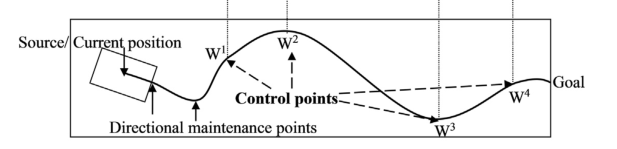
\includegraphics[width=0.8\linewidth]{kalaBezier.png}
        \caption{Bézier curves for route representation from Kala \cite{kalaOnroadIntelligentVehicles2016}}%
        \label{fig:.ext}
    \end{figure}

    \begin{itemize}
        \item A Bézier curve with $n$ control points is said to have a \textit{degree} of $n-1$ (initial point is called $P_0$ and is not counted in degree)
        \item A Bézier with a degree of 1 is a straight line between the two control points (the start and end point)
        \item Further control points \textit{bend} the line into a curve.
        \item The curve does not necessarily pass through all intermediate control points but it is determined by them.
        \item Bézier curves are smooth $\implies$ good for representing vehicle routes
        \item Trivially, they are also continuous so will represent an entire route from $A \rightarrow B$ 
    \end{itemize}
\end{frame}

\begin{frame}

    \note{

        \begin{itemize}
            \item Bézier curves are parametric in nature, so therefore work well with parameter based optimisation techniques such as Genetic Algorithms. 
            \item We can represent the control points as genes in each genome
            \item We can map the fitness of a curve to its length in feasible space.
        \end{itemize}

    }

    \begin{itemize}
        \item By their definition, Bézier curves are parametric. This lends themselves nicely to an parametric optimisation techniques such as GAs.
        \item We can represent the control points as genes in the genome of each candidate.
        \item We can represent a curve's fitness as its length within feasible space.
    \end{itemize}
\end{frame}

\begin{frame}
    \note{

        Here you can see my implementation of bezier curves as routes being drawn in an implementation of the road coordinate system mentioned earlier.

    }
    \begin{figure}[htpb]
        \centering
        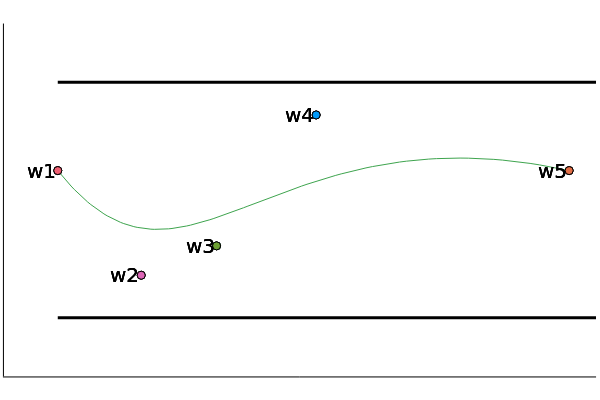
\includegraphics[width=0.8\linewidth]{bezierdemo.png}
        \caption{Example of Bézier curve of degree 4 in road coordinate space, my implementation}%
        \label{fig:bezierdemo}
    \end{figure}
\end{frame}

\section{Methods}

\begin{frame}{Methods}

    \note{

        \begin{itemize}
            \item I have begun my project by looking into the current research. I have read and collated paper surrounding the subject of GAs and vehicle routing problems.
            \item In doing so, I have found substantial research into GAs generally, but relatively little on their applications on fully autonomous road networks; with the bulk of the available research being from Rahul Kala from the Indian Institute of Information Technology.
            \item I have also started the implementation phase of my project.
            \item Using the programming language Julia, I have implemented the Bézier curve function, types for various GA structures, plotting utilities for visualising the problem and the basic initialisation function for the GA
            \item These are likely not the final versions but seem to perform well.
        \end{itemize}

    }

    I have started by reading and collating papers, books and articles surrounding GAs and their applications on routing problems.

    I have found substantial research into GAs but only a few papers on my sub-area, mainly by Rahul Kala from the Indian Institute of Information Technology.

    I have begun implementing various utility functions and types in Julia\cite{JuliaProgrammingLanguage}, including:

    \begin{itemize}
        \item Bézier curve functions
        \item Road, Individual, Phenotype and Genotype types
        \item Plotting utilities for Roads and candidate solutions
        \item Population initialisation functions
    \end{itemize}

    Still to implement: 

    \begin{itemize}
        \item Genetic operators
        \item Cooperative route planning wrapper
    \end{itemize}

\end{frame}
\begin{frame}

    \note{
    
        \begin{itemize}
            \item Once the basic shape of the GA is implemented, the main focus of my project can begin. 
            \item Here I will begin to experiment with a variety of variable and parameter values, as well as different genetic operators such as different point crossover techniques and stochastic sampling. 
            \item In my report I will evaluate these different approaches and attempt to conclude which perform best 
            \item Genetic algorithms can also have heuristics baked into them similar to the process of converting Djikstra's algorithm to $A^*$ 
        \end{itemize}

    }

    Once a basic GA has been implemented, the stage of variable and operator refinement can begin.
\\~\

    There are many oppertunities for improvement of GAs with a wide variety of crossover and mutation techniques being discussed in literature, each performing differently depending on the search space.
\\~\

    One aim of my report will be to assess and collate the effectiveness of a wide variety of such operators, with the hope of concluding which are best for the task. 

    GAs can also be augmented via the use of domain-specific heuristics and as such I will investigate this area also
\end{frame}

\section{Bibliography}
\begin{frame}[allowframebreaks]
\frametitle{References}
\bibliographystyle{abbrv}
\bibliography{lib}
\end{frame}

\end{document}
